
\documentclass[a4paper]{report}

% bibliography
\usepackage{natbib}
%\bibpunct{[}{]}{,}{a}{}{;}

\usepackage{fancyheadings}
\usepackage{iamdip}
\usepackage[pdftex]{graphicx}
% ignore missing images
%\usepackage[demo]{graphicx}
\usepackage[labelfont=bf, font={sf,normalsize}, margin=0.5cm]{caption}
\usepackage{caption}
\usepackage{subcaption}
\usepackage{amsmath}
\usepackage{amssymb}
\usepackage{amsfonts}
\usepackage{url}
\usepackage{hyperref}
\usepackage{listings}
\usepackage{chngpage}

% For notation table
\usepackage{tabulary}
\usepackage{booktabs}

\usepackage{here}

\headrulewidth 0.5pt \addtolength{\headheight}{5pt}
\lhead[\fancyplain{}{\rm\thepage}]{\fancyplain{}{\rightmark}}
\rhead[\fancyplain{}{\leftmark}]{\fancyplain{}{\rm\thepage}}
\cfoot{}

\graphicspath{{Figures/}}

\newcommand{\T}{^\text{T}}

% for fancy todo
\usepackage{todonotes}
\newcommand{\todoRef}{\todo[color=green!20]}
\newcommand{\todoEnglish}{\todo[color=red!20]}
\newcommand{\todoFormat}{\todo[color=blue!20]}
\newcommand{\todoWriteMore}{\todo[color=yellow!40, inline]}
\newcommand{\todoRewrite}{\todo[color=purple!20, inline]}
\newcommand{\todoQ}{\todo[color=blue!20]}

% math definitions, propositions and such
\usepackage{amsthm}
\newtheorem*{definition}{Definition}
\newtheorem*{rules}{Rules}
\newtheorem*{example}{Example}
\newtheorem{assertion}{Assertion}

% tree packages and basic settings
\usepackage{tikz}
\usetikzlibrary{arrows,shapes,positioning,shapes.geometric,fit}
\usepackage{xcolor}
\tikzset{
treenode/.style = {align=center, inner sep=0pt, text centered,
font=\sffamily},
arn_n/.style = {treenode, circle, white, font=\sffamily\bfseries, draw=black,fill=black, text width=1.5em},% arbre rouge noir, noeud noir
arn_r/.style = {treenode, circle, red, draw=red, text width=1.5em, very thick},% arbre rouge noir, noeud rouge
arn_w/.style = {treenode, circle, draw=black, text width=1.5em, very thick},% arbre rouge noir, noeud rouge
arn_x/.style = {treenode, rectangle, draw=black, minimum width=0.5em, minimum height=0.5em},% arbre rouge noir, nil
subtree/.style  = {regular polygon, regular polygon sides=3, draw=black, align=center, minimum size=1cm, anchor=center}
}

%%%%%%%%%%%%%%%%%
% begin document
\begin{document}

\pagestyle{fancyplain} \thispagestyle{empty}

\title{Justification Proof Search Implementation in Python}
\author{Judith Fuog}
\betreuer{Prof.\ Dr.\ Thomas Studer}
\ort{Bern}
\datum{2014}


\pagenumbering{roman} \setcounter{page}{1}
\maketitle

\newpage
\thispagestyle{empty}
\vspace{8cm}
\noindent
{\centerline {\bf \large Abstract}}
\vspace{1cm}

\noindent In short what's it all about.

\pagenumbering{roman} \setcounter{page}{1}
\tableofcontents

%Introduction
%	Motivation
%	Goal
%	Overview
%
%Background
%	Justification Logic
%	Operation Tree 
%
%Algorithm: A Divide and Conquer Approach
%	Core Idea
%	Divide
%		Atomize
%			Sumsplit
%			Simplify
%			Remove Band Bang
%		Get Must
%	Conquer
%		Congifurations and Conditions
%		Merge
%	Implementation
%
%Result
%	Application
%	Enhancement

\newpage{\pagestyle{empty} \cleardoublepage}

% Hauptdokument
\pagenumbering{arabic} \setcounter{page}{1}
\pagestyle{fancy}


\chapter{Introduction}
\section{Motivation}
\section{Goal}
\section{Overview}


\chapter{Background}
\section{Justification Logic}
\section{Order of Operation Tree}




\newpage{\pagestyle{empty} \cleardoublepage}
\chapter{A Divide and Conquer Algorithm}
\label{chap: Algorithm A Divide and Conquer Approach}

\section{Core Idea}



\section{Divide}
\subsection{Atomize}
\subsubsection{Sumsplit}
\subsubsection{Simplify Bang}
\subsubsection{Remove Bad Bang}
\subsection{Get Must}

\section{Conquer}
\subsection{Configurations and Conditions}
\subsection{Merge}

%!TEX root = ../bachelors_thesis.tex
\begin{example}
\[
	((((a*b)*(!b))+((!b)+c))+((!b)*d)):(b:F)
\]
\end{example}
%!TEX root = ../bachelors_thesis.tex

\section{Model Overview}
For the implementation of this algorithm there was only one model that truly stood out in the sense of object orientated programming. For all other functions it proved rather difficult to find a clear class where it belonged to and also making good use of responsibilities of those classes. As mentioned in chapter \ref{chap: Justification Logic} the main work was done using syntax trees and so it was the most obvious class to build. I decided to make a extra class for the \emph{Nodes} where all the small things like setting a child, and checking if it is a root and such would be handled. \emph{Tree} and \emph{Node} could have been merge to be one class only but I found it easier to work with the code if the more standard and trivial stuff of binary trees was separated from what was more specific for this algorithm. A lot of the \emph{atomize} part is handled by the \emph{Tree} class since it works within the formula and also changes the structure of it.

The most important class however is the \emph{ProofSearch} class. It acts as a sort of main class as the initialization of the formula and the cs-list takes place here. It is also here that the methods of the \emph{Tree} class are called from. Its responsibility is to handle all algorithmic task that can be done without using a syntax tree. So the major logic of the conquer step is implemented here.

Last there is the typical \emph{Helper} class. The methods here are usually rather short  and simple and serve the purpose of making the \emph{Tree} and \emph{ProofSearch} class appear cleaner. It may be argued that some of those methods present in \emph{Helper} should be better placed in \emph{ProofSearch} and vice a verse but then again the argument for a clean object orientated model design for an algorithm is questionable and very difficult to archive.

\begin{figure}[H]
	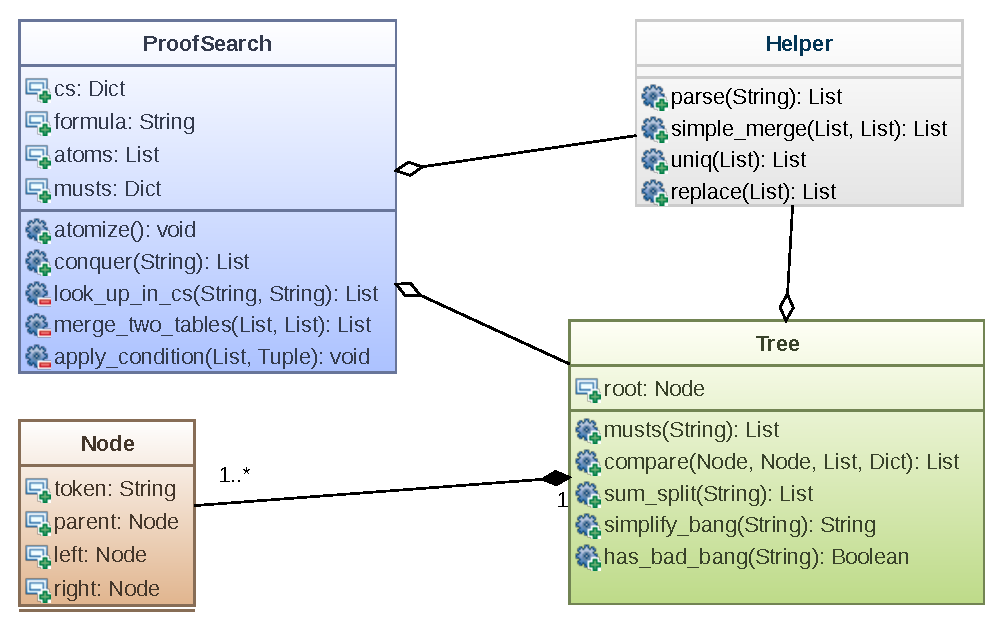
\includegraphics[width=0.9\textwidth]{/home/lyriael/BA/j-logic/thesis/Figures/uml_01.pdf}
	\caption{Simplified UML graphic of the classes used for implementing the algorithm. The list of methods and attributes is by no means complete and should simply give an idea of the construction.}
	\label{uml}
\end{figure}

\section{Operation Syntax Tree}
One of the earliest challenges was a useful representation of a formula with which I could work decently. Interestingly enough a binary tree came only later into my mind, after I tested various libraries from Python. There were libraries that seemed very useful at first as they were math-specific. Analyzing formulas that contained $*$ or $+$ were fairly easy but as $:$ and $!$ are not very common operations I could not customize the tested libraries enough to handle those as well.

So it happened while I was searching yet for another library that I tumbled over the possibility to use binary trees to represent the syntax of a mathematical formula. Remembering a lot of what I learned in the lecture about Datastructure and Algorithms I realized that this is the best choice for me. A binary tree gives me not only a way to represent a formula in a way that interprets the order of operations but with the knowledge about trees it became suddenly very easy to also manipulate such a formula for example by deleting or swapping subtrees and still keep a valid operation. 

I decided to implement my own tree for that purpose. It might be argued that a lot of work could be saved if I used available syntax trees but for one thing I relished the idea of implementing a tree structure that I would use myself and thus finally use what I have learned in lecture ages ago and second I would have to make custom changes to a finished solution anyway and those changes are probably more work than the implementation of a binary tree which is rather simple.

I tried to keep the tree as simple as possible, giving the nodes only a value and not a unique key. The greatest challenge given by implementing a syntax tree was to handle the unary operator $!$. As braces serve to determine the depth of a tree and a binary operation tells you when to start climbing up again, it required so extra case handling for the $!$ operator. From the point on when the tree was working, it was not only important to the algorithm, but could also be used to check if the input was written correctly. Therefore most of the tests that test the string handling of a tree are the result of formulas used somewhere else but which needed syntax spell checking. 


\section{Important Methods}
In this section I want to show and explain some of the more complicated methods that are important and make up the heart of the algorithm.

\subsection{Tree.musts}
The method \emph{musts} expects a given proof term to be already \emph{atomized} as it only distinguishes between $!$ and $*$ operations.
The algorithm takes the formula in form of a tree apart from top to bottom, generating new, smaller terms for every operation it takes apart until the remaining proof term is only a proof constant. Since the resolve of a $*$ operation needs a new \emph{X-wild} and the resolve of a $!$ operation replaces an existing \emph{x-wild} and therefore needs a new as well, the current $i$ for a new \emph{X-wild} $X_i$ is stored and increased in \texttt{v\_count}.

\begin{figure}[H]
    \vspace{-10pt}
	\lstinputlisting[firstline=2, lastline=22]{/home/lyriael/BA/j-logic/thesis/code_tree.py}
	\vspace{-10pt}
	\caption{Excerpt from $Tree.musts$}
	\vspace{-10pt}
\end{figure}

If for example the current justification term would be $((a*(!b)):F)$, it would be taken apart to the two subformulas $(a:(X_i\rightarrow F))$ and $((!b):(X_i))$. Because of the \emph{atomization} in the steps before it is guaranteed that every $!$ is a (right) child of a  $*$ and since every $*$ creates a new $X_i$, a term here that starts with a $*$ is always on a $X_i$. Since from $!b:X_i$ follows $\exists X_j \quad s.t. \quad !b:(b:X_j)$, all $X_i$ that occurred up to now must be replaced by $(b:X_j)$. In the end we will have only proof constants remaining.

\subsection{Tree.compare}
This method gives us foundation to the method \emph{apply\_condition} which we will look at later. It is also only very tedious and was probably written and rewritten again more than any other part of the code. It basically compares the value of each node of a tree with the corresponding value of a node of another tree. As long as the token (value) of the nodes are the same it will just process, but in case the two nodes are not identical several cases will be distinct.


\begin{figure}[H]
	\vspace{-10pt}
	\lstinputlisting[firstline=24, lastline=38]{/home/lyriael/BA/j-logic/thesis/code_tree.py}
	\vspace{-10pt}
\end{figure}
\begin{figure}[H]
	\vspace{-10pt}
	\lstinputlisting[firstline=41, lastline=46]{/home/lyriael/BA/j-logic/thesis/code_tree.py}
	\vspace{-10pt}
	\caption{Excerpt from $Tree.compare$}
	\vspace{-10pt}
\end{figure}

If the current node of the term from the cs-list has a \emph{Y-wild} all other occurrences of this \emph{Y-wild} within this term will be replaces with whatever node or subtree is found in the term of the \emph{musts}. As a consequence it is possible to find a \emph{X-wild} within the term from the cs-list. Whenever that is the case, the value found in the node/subtree of the term of the \emph{musts} is a condition to this $X_i$. If the condition is merely a constant value, it will be set directly.

As can be seen here the return value of this method is a list of conditions and a dictionary containing the found wilds. If a contradiction is found during the comparison both will be set to \texttt{None} rather than being returned empty, since it is possible that a comparison need neither conditions nor wilds but still works.
\todoWriteMore{Graphic with wild replacement for compare method}

\subsection[ProofSearch.apply\_conditions]{ProofSearch.apply\_condition \\and ProofSearch.apply\_all\_conditions}
These methods are called from within the method \texttt{full\_merge\_of\_two\_configs} if the wilds of the configurations can be merged. It is used to make sure that the new found configuration still holds for all conditions that applied before to each of the old configurations before they were merged.

This again proved more difficult than expected so I split it in two methods where the first simply handles one condition on one term and the other method makes sure that all conditions are taken care of. In the cases I studied so fare there is usually only one condition to a configuration but since it is possible that a configuration holds several conditions the method must hold in those cases as well.

\subsubsection{Apply One Condition}
The input arguments given to the method are the merged configuration and one condition tuple.

\begin{figure}[H]
	\vspace{-10pt}
	\lstinputlisting[firstline=1, lastline=3]{/home/lyriael/BA/j-logic/thesis/code_proof_search.py}
	\vspace{-10pt}
	\caption{Excerpt from $ProofSearch.apply\_condition$.}
	\vspace{-10pt}
\end{figure}

Since a condition is always on one $X_i$ the term we find in the configuration for $X_i$ is of high interest. But because the condition term may also contain other $X_j$ we need the whole configuration and not only the term on which the condition is. If there is now term for $X_i$ in the configuration yet the condition cannot be applied and must be kept for later reference. 

In the case that we do find an entry for $X_i$ in the configuration it will be compared with what we have in the condition term.

\begin{figure}[H]
	\vspace{-10pt}
	\lstinputlisting[firstline=8, lastline=25]{/home/lyriael/BA/j-logic/thesis/code_proof_search.py}
	\vspace{-10pt}
	\caption{Excerpt from $ProofSearch.apply\_condition$.  }
	\vspace{-10pt}
\end{figure}

Generally spoken there are three outcomes for a condition when it is checked against the merge of two configurations.

\begin{itemize}
	\item The condition is in contradiction with the merge of the two configurations. The merge is abandon and not further considered.
	\item The condition holds against the new merge but a comparison gave use \emph{X-} and/or \emph{Y-wilds}.
	\begin{itemize}
		\item Found \emph{X-wilds} will be written into the configuration merge.
		\item Found \emph{Y-wilds} will be passed on to be handled later on.
	\end{itemize}
	\item The condition holds against the new merge and no \emph{wilds} emerged. The condition is discarded since it is not used anymore.
\end{itemize}

\subsubsection{Apply All Conditions}
Applying all conditions instead of just one should be straight forward but I found it more difficult than expected. Since the number of conditions may change during iteration and since it is also possible that a condition that held a \emph{Y-wild} can change and has to checked again, a simple \texttt{loop} would not do.

\begin{figure}[H]
	\vspace{-10pt}
	\lstinputlisting[firstline=36, lastline=58]{/home/lyriael/BA/j-logic/thesis/code_proof_search.py}
	\vspace{-10pt}
	\caption{Excerpt from $ProofSearch.apply\_condition$. The  }
	\vspace{-10pt}
\end{figure}


If the condition can be satisfied the variable \texttt{updated\_config} will be true for the \texttt{if}-query. If a condition is still returned it must be kept for later reference thus. If \texttt{Y-wilds} contains any entries all conditions that contain any of the wilds (even those that have been checked already) will be updated and checked again. This is for the case that a \emph{Y-wild} has been found and although a \emph{Y-wild} may stand for any term, it must be the same term for all $Y_i$. 

The \texttt{break} in the code indicates the situation that one of the conditions could not be satisfied thus the whole merge is a fail. 

\subsection[ProofSearch.merge]{ProofSearch.full\_merge\_of\_two\_configs \\and merge\_two\_tables}
Similar as in the previous section the process that uses the methods above and actually merges all configurations together to get a solution is split in two parts where the first part handles a merge of only two configurations and the other handles the full merge.

\subsubsection{Simple Merge}
The actual merge is a very simple method found in the \texttt{Helper} class. It simply checks if the two given lists contain the same \texttt{String} or if at least one of the items in the list is an empty \texttt{String}.

\subsubsection{Full Merge of Two Configs}


\section{Tests}
\todoWriteMore{Todo}


%\newpage{\pagestyle{empty} \cleardoublepage}
%
%\input{Content/guidedImageFiltering}
%
%\newpage{\pagestyle{empty} \cleardoublepage}

%!TEX root = ../bachelors_thesis.tex
\todoWriteMore{Todo}
\section{Application}
\section{Enhancement}

 
%\addcontentsline{toc}{chapter}{\numberline{}List of Tables}
%\listoftables

%\addcontentsline{toc}{chapter}{\numberline{}List of Figures}
%\listoffigures
\addcontentsline{toc}{chapter}{\numberline{}Bibliography}
\bibliographystyle{plainnat}
%\bibliographstyle{plain}
\bibliography{sources}
%\bibliographystyle{alphadin}
\nocite{*}

\newpage{\pagestyle{empty} \cleardoublepage}
%\chapter*{Authorship}
\listoftodos

\end{document}